\section{Auditor Extension} \label{sec:auditor}
Until now we have not \emph{verified} whether the certificate chain of an SFO is
publicly logged as promised by the issued SCTs.  As such, it is unlikely that a
misbehaving CT log will be detected.
Our base design can be extended to follow-up
on an SFO's inclusion status rather than adding the underlying certificate chain
to another CT log.  This has the benefit of relaxing our initial trust
assumption, namely that some CT logs are honest, as well as making it possible
to disclose those CT logs that are dishonest.  The downside is added
complexity, which introduces additional threats that must be considered.

\subsection{Design Sketch} \label{sec:auditor:design}
Figure~\ref{fig:auditor} provides an overview of the extended design.  Tor
Browser submits presented SFOs probabilistically to CTRs that are selected at
random, and CTRs store the submitted SFOs before any auditing takes place.
Here, auditing refers to inclusion verification rather than adding certificate
chains.  The moment before auditing, the SFO in question is shared with a CTR
that acts as a \emph{watchdog}.  Unless the auditing CTR receives a timely
inclusion proof and acknowledges it to its watchdog, the (now suspicious) SFO is
reported to a CT auditor.  Phase~1 remains unchanged, some changes are needed
in phase~2, and major changes are required in phase~3 as well as the Tor
consensus.  The extra-info document also includes two new metrics that are
related to flooding.
%Another prerequisite is the existence of CT auditors.

\begin{figure*}
    \centering
    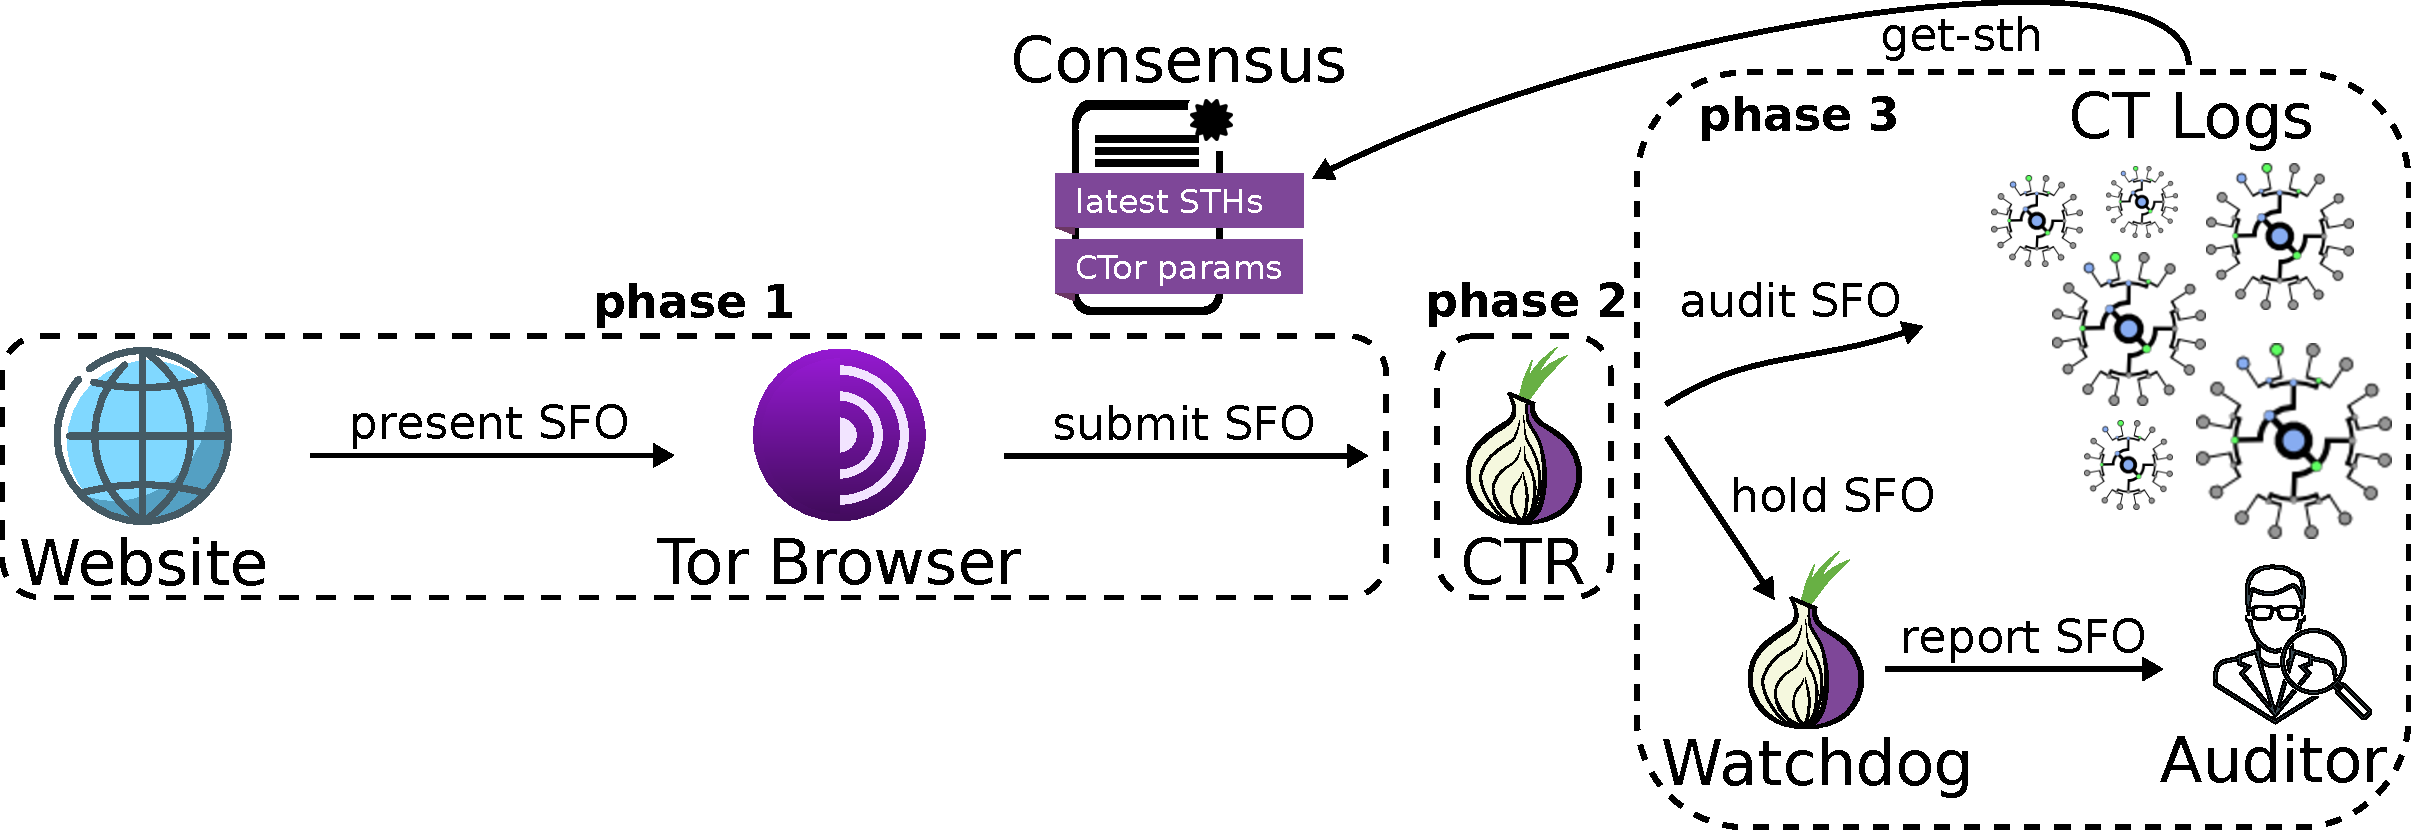
\includegraphics[width=0.85\textwidth]{img/design-auditor}
	\caption{The auditor extension to CTor, where cryptographic evidence of log
	omission can be collected without modification to CT logs. The extension
	changes the consensus to include the latest STHs from CT logs and makes
	phase 3 significantly more complex. CTRs in phase 3 now challenge logs to
	prove inclusion of certificates from SFOs, using other CTRs as
	``watchdogs'', ensuring that SFOs that are not provably correct are reported
	to trusted auditors.}
	\label{fig:auditor}
\end{figure*}

\subsubsection{Tor Consensus} \label{sec:auditor:design:consensus}
Tor's consensus should capture a fixed view of the CT landscape by publishing
STHs from all recognized logs.  A CT log is recognized if a majority of directory
authorities proposed a \texttt{ct-log-info} item, which contains a log's ID,
public key, base URL, MMD, and most recent STH.  Note that each directory
authority proposes its own STH, and agrees to use the most recent STH as
determined by timestamp.  Since CTRs verify inclusion statuses of SCTs
that Tor Browser accepts, the CT logs recognized by Tor Browser must be in
Tor's consensus.

Tor's directory authorities also majority-vote on \texttt{ct-auditor} items,
which pin base URLs and public keys of CT auditors that watchdogs contact in
case that any log misbehavior is suspected.  A watchdog triggers if the time
specified by \texttt{ct-watchdog-timeout} elapses without receiving any
acknowledgment.  The following auditor submission is governed by a
\texttt{ct-auditor-timeout}, which, if triggered, results in a resubmission
later on.

\subsubsection{Phase~2---Storage} \label{sec:auditor:design:phase2}
Other than updating the criteria of what it means that an SFO can be audited
in phase~3, the computation of $l$ and $t$ changes for a buffer's entry.  With
regards to some CT circuit, process an incoming SFO $s$ as follows:
\begin{enumerate}
	\item\label{enm:ext:storage:close} Close the current circuit to enforce
		one-time usage.
	\item\label{enm:ext:storage:unrecognized} Discard unrecognized SCTs in $s$
		whose logs have no corresponding \texttt{ct-log-info} items listed in
		the Tor consensus.  Stop if there are no remaining SCTs in~$s$.
	\item\label{enm:ext:storage:cached}
		Stop if $s$ is cached or pending to be audited already.
	\item\label{enm:ext:storage:fix-log} Sample a CT log $l$ that issued a
		remaining SCT in~$s$.
	\item\label{enm:storage:audit-after} Compute an \texttt{audit\_after}
		time~$t$, see Figure~\ref{fig:audit-after}.
	\item\label{enm:storage:store} Add $(l,t,s)$ to a buffer of pending SFOs.
\end{enumerate}

Recall from Section~\ref{sec:background:ct} that an inclusion proof is fetched
with regards to an STH.  As such, we discard SCTs that cannot be verified due to
lack of \texttt{ct-log-info} items in the Tor consensus.  The sampled CT log $l$
now refers to an entity that issued an SCT in the submitted SFO, and it will be
challenged to prove inclusion in phase~3 sometime after the
\texttt{audit\_after} timestamp $t$ elapsed.  Figure~\ref{fig:audit-after} shows
that $t$ takes the log's MMD into account.  This is one of two parts that
prevent \emph{early signals} to the issuing CT logs that an SFO is being
audited.  For example, if an SFO is audited before the MMD elapsed, the issuing
CT log could simply merge the underlying certificate chain to avoid an MMD
violation.  This would not yield any improvement with regards to the base
design.

\begin{figure}
	\centering
	\pseudocode[linenumbering, syntaxhighlight=auto]{%
		\textrm{t} \gets \mathsf{now}() +
			\mathsf{MMD} +
			\mathsf{random}(\texttt{ct-delay-dist}) \\
		\pcif \textrm{SCT.timestamp} + \textrm{MMD} <
				\mathsf{now}():\\
			\pcind\textrm{t} \gets \mathsf{now}() +
				\mathsf{random}(\texttt{ct-delay-dist})
	}
	\caption{%
		Algorithm that computes an \texttt{audit\_after} timestamp $t$.
	}
	\label{fig:audit-after}
\end{figure}

\subsubsection{Phase~3---Auditing} \label{sec:auditor:design:phase3}
In addition to maintaining a single Tor circuit that is used to interact with
CT logs that have \texttt{ct-log-items}, a distinct Tor circuit is maintained
and rotated that ends at a random watchdog CTR.  Given a known CT log
$l$:
\begin{enumerate}
	\item\label{enm:ext:auditing:backoff} Sample a delay $d \gets
		\mathsf{random}(\texttt{ct-backoff-dist})$.
	\item\label{enm:ext:auditing:sleep} Schedule a timer, waiting until $d$
		time units elapsed.
	\item\label{enm:auditing:loop} For each pending buffer entry $(l',s,t)$:
		\begin{enumerate}
			\item\label{enm:ext:auditing:log-check}
				Continue the loop if $l\ne l'$.
			\item\label{enm:ext:auditing:timestamp-check} Continue the loop if
				$t > \mathsf{now}()$.
			\item\label{enm:ext:auditing:sth-check} Continue the loop if $t >
				\textrm{STH}.\mathsf{timestamp}$.
			\item\label{enm:ext:auditing:watchdog} Share $s$ with the current
				watchdog.
			\item\label{enm:ext:auditing:challenge} Use \texttt{ct-log-timeout}
				and $\textrm{STH}.\mathsf{treesize}$ to set a timer and
				challenge the log to prove inclusion.
				\begin{itemize}
					\item\label{enm:ext:auditing:challenge:success} On valid
						proof: send an acknowledgment to the watchdog, then
						cache $s$ and discard it.
					\item\label{enm:ext:auditing:challenge:fail} On any other
						outcome: discard $s$ and break.
				\end{itemize}
		\end{enumerate}
	\item\label{enm:ext:auditing:restart} Go back to
		step~\ref{enm:ext:auditing:backoff}.
\end{enumerate}

An SFO is not audited for inclusion until the log's MMD elapsed \emph{and} there
is an STH in the Tor consensus that captures it.  As such, a CT log that intends
to omit a certificate chain despite promising to merge it within its MMD will
not get an early signal that a CTR will audit it.
Before auditing, the SFO in question is shared with a watchdog that takes on
the responsibility of reporting suspicious SFOs to the pinned CT auditors.
An SFO is considered suspicious if it is not acknowledged by the log-challenging
CTR as verified within the time specified by \texttt{ct-watchdog-timeout}.  As
argued in Section~\ref{sec:auditor:analysis:phase3}, it is motivated to use a
watchdog:
	the attacker learns which CTR holds the problematic SFO at the time of
		auditing, and
	during the \texttt{ct-log-timeout} actions could then be taken to ensure
		that the SFO does not reach a CT auditor.
A watchdog that receives a suspicious SFO reports it to a random CT auditor,
and resubmits it later on if the \texttt{ct-auditor-timeout} happens to trigger.

\subsubsection{Extra-Info Document} \label{sec:auditor:extra-info}
Following from the \texttt{audit\_after} timestamp algorithm in
Figure~\ref{fig:audit-after}, an SFO may be stored throughout an entire MMD.
This results in a relatively large time window during which the attacker can
attempt to flood all CTRs in hope that they delete the omitted SFO at random
before it is audited.  We discuss the threat of flooding further in
Section~\ref{sec:auditor:analysis:phase2}, noting that it can be detected if
CTRs publish two new metrics in the extra-info document:
	\texttt{ct-receive-bytes} and
	\texttt{ct-delete-bytes}.
These metrics indicate how many SFO bytes were received and deleted throughout
different time intervals, which is similar to other extra-info metrics such
as \texttt{read-history}.

\subsubsection{CT Auditor} \label{sec:auditor:auditor}
An announced auditor is expected to accept SFOs at a dedicated endpoint,
endeavoring to validate the inclusion status of each SCT with regards to the
first STH in the Tor consensus that elapsed the log's MMD.  If a log appears to
function correctly except for some evidence that cannot be
resolved despite multiple attempts that span a given time period, it is
paramount that the auditor software alerts its operator who can investigate
the issue further before submitting a full report to the CT-policy mailing list.
Cases of misbehavior, in detail:
\begin{itemize}
	\item If the log fails to provide a valid inclusion proof for an SCT with
		regards to the first applicable STH in the Tor consensus
		(certificate omission).
	\item If the log fails to provide a valid consistency proof between two
		STHs in the Tor consensus
		(split-view).
	\item If a published STH is future-dated or backdated more than an MMD
		(general log misbehavior).
	\item If a log ignores some CTRs (uptime misbehavior).
\end{itemize}

An unresponsive log can be suspected by observing the watchdog report frequency,
and possibly confirmed by querying the log in question from different vantage
points.  Among other extra-info metrics that go beyond received and deleted
SFO-bytes that the announced CT auditors should check, it could be valuable to
publish the extent to which CTR-to-log interactions fail.

%While not within our threat model, we do encourage the announced auditors to
%verify that STHs in the Tor consensus are consistent with external views of the
%CT landscape.  For example, operate an STH pollination~\cite{nordberg} endpoint
%and fetch STHs actively from many diverse vantage points using Tor, VPN
%services, DoH resolvers, and RIPE Atlas (to mention a few low-cost options).
%This goes back to the point of general ecosystem value.
% => this is now a "forward point"

\subsection{Security Analysis} \label{sec:auditor:analysis}
Idea: go through what is \emph{different} with regards to the base analysis.

Make sure it is clear why we do delete at random before analysis starts

Have to hand-wave a few obvious things before we get started, e.g., maybe the
attacker controls some announced auditors, but not all so it is not reliable.

\subsubsection{Phase~2---Storage} \label{sec:auditor:analysis:phase2}
The main difference with regards to the base design is that an SFO can be
stored much longer.  The attacker can maximize the \texttt{audit\_after}
timestamp by using a newly issued SFO, resulting in a storage phase of \emph{at
least} an MMD.  This time can be extended further by delaying issuance of an
STH that would capture the omission:
	a log must produce an STH every MMD~\cite{ct,ct/bis}.
This means that the maximized storage time is in the order of two MMDs; not
considering that it also takes time for an STH to be propagated into the Tor
consensus.  Most logs use an MMD of 24~hours, resulting in an attack window that
ranges from one to two days.  A risk-averse attacker should prefer to use the
lower bound:
	suddenly not issuing any new STH is visible, attracting attention.

Following from Tor's threat model, the mis-issued SFO must be stored in
volatile memory and not to disk.  Two risks emerge as a result of the increased
storage time:
	the CTR in question might be restarted by the operator,
	and the attacker might \emph{flood} it by submitting many SFOs with the
		intent to \emph{flush} a target entry from the buffer~\cite{nordberg}.
A risk-averse attacker cannot rely on the former, but the latter is applicable
if all CTRs can be targeted without making Tor unavailable.
Appendix~\ref{app:flush} shows that the number of SFO submissions~$k$
that the attacker needs to successfully flush a buffer of $n>1$ entries with
some probability~$p<1$ is given by Equation~\ref{eq:flush}.
\begin{equation} \label{eq:flush}
	k = \frac{\log(1-p)}{\log(1 - \frac{1}{n})}
\end{equation}

It is recommended that a non-exit relay should have at least 512~MB of memory.
If the available bandwidth exceeds 40~Mbps, it should have at least
1~GB~\cite{relay-config}.  Given that these recommendations are lower bounds,
suppose the average memory available to store SFOs is 1~GiB.  Further, our
dataset in Section~\ref{sec:performance} shows that the average SFO is in the
order of 6~KiB.  This means that the buffer capacity is $n \gets 174763$ SFOs.
Plugging it into Equation~\ref{eq:flush} for $p \gets \frac{9}{10}$, the
attacker's flood must involve $k \gets 402406$ submissions.  In other words,
2.3~GiB must be transmitted to flush a single CTR,\footnote{%
	As a corner case and implementation detail, it is important that Tor Browser
	and CTRs \emph{reject} SFOs that are bogus in terms of size:
		it is a trivial DoS vector to load data indefinitely.
	Analysis based on, e.g., 1~MiB SFOs also requires 2.3~GiB of data to flush.
} which takes $7.9$--$39.3$~minutes if its bandwidth is between 8 and 40~Mbps.
Thus, it is impractical to flush all CTRs within minutes.

Metrics reported by the Tor project show that there are over 4000 relays that
match our CTR criteria~\cite{relay-by-flag}.  As such, a network-wide flush
involves the transmission of at least 8.99~TiB.  It might sound daunting at
first, but distributed over a day it only requires 0.91~Gbps.  While we cannot
avoid early signals to the logs \emph{and} at the same time prevent flushing
without writing anything to disk, it is detectable based on the extra-info
document.  On the flip-side, \emph{not observing any flushing} adds a large
degree of confidence that there are no mis-issued SFOs.

\subsubsection{Phase~3---Auditing} \label{sec:auditor:analysis:phase3}
The main difference with regards to the base design is that we query the
attacker for inclusion proofs; not an independent CT log.  As such, there is a
time window to act between the time that the attacker learns some CTR audits a
mis-issued SFO and until the \texttt{ct-log-timeout} elapses.  Suppose that the
attacker could identify the CTR in question at the time of auditing, i.e.,
despite our design (re)using a Tor circuit for all inclusion proofs.  Clearly,
the query timeout must be a few seconds to avoid premature auditor reporting.
This leaves a large enough window to simply DoS the CTR in question.  Our design
makes no attempt to hide the CTR's identity while querying the log.  For
example, the attacker can trivially \emph{tag} each CTR by submitting many
distinct SFOs, and upon seeing them in the audit loop the exact identity is
revealed.  We mitigated this threat using a watchdog, sending the SFO upfront
\emph{before} auditing.  The attacker does not know the watchdog identity based
on the same premises that the attacker does not know which CTR stores an
SFO during the storage phase.

Another difference is that inclusion proofs are based on STHs that the directory
authorities fetch from attacker-controlled CT logs, agreeing on which ones to
use via deterministic rules.  This means that the attacker controls which STHs
go into the Tor consensus.  Once an STH is announced, it follows from Tor's
threat model that it is fixed because a threshold of directory authorities are
benign.  As such, CTRs have access to the same (in)consistent view of the CT
landscape.  Fortunately, any inconsistent view that makes it into the Tor
consensus is trivially detected:
	the announced STHs are public and auditable by anyone.
Therefore, the attacker should be deterred from creating split-views in Tor.
Other user agents could benefit from Tor's audited view of CT logs.

% MISC notes
% - Network-wide flush, detectable but hard to attribute
% - Requires new reliable auditor software
% - Bit more bandwidth due to watchdog.  The overhead, when compared to log a
% log extension, is sending an SCT hash and receiving a proof (2-3KiB).
% - A rational attacker is the issuer of all SCTs in the omitted SFO, so it is
% sufficient to verify inclusion with regards to one SCT and then leave it to
% the auditors to bust all involved CT logs.
